\documentclass[epsfig,10pt,fullpage]{article}

\newcommand{\LabNum}{9}
\newcommand{\CommonDocsPath}{../../../../common/docs}
\addtolength{\textwidth}{1.5in}
\addtolength{\oddsidemargin}{-0.75in}
\addtolength{\topmargin}{-0.75in}
\addtolength{\textheight}{1.5in}
\addtolength{\evensidemargin}{0.75in}
\setlength\parindent{0pt}
\raggedbottom

\usepackage{ae,aecompl}
\usepackage{epsfig,float,times}
\usepackage[hypcap]{caption}
\usepackage[pdftex, colorlinks]{hyperref}
\usepackage{graphicx}
\usepackage[usenames, dvipsnames]{color}
\usepackage{rotating}
\usepackage{tikz}
\usetikzlibrary{automata,positioning}
\usepackage{placeins}

\widowpenalty 10000
\clubpenalty 10000

\newcommand{\red}[1]{{\color{red}\sf{#1}}}
\newcommand{\green}[1]{{\color{green}\sf{#1}}}
\newcommand{\blue}[1]{{\color{blue}\sf{#1}}}
\definecolor{PineGreen}{rgb}{0.0, 0.47, 0.44}
\definecolor{ForestGreen}{rgb}{0.13, 0.55, 0.13}
\definecolor{Brown}{rgb}{0.59, 0.29, 0.0}

\newcommand{\UPDatePublished}{Oct 2021}
\newcommand{\versnum}{21.1} %version number quartus/AMP
\newcommand{\quartusname}{Quartus\textsuperscript{\textregistered} Prime}	
\newcommand{\UPTextBar}{For \quartusname{} \versnum{}}
\newcommand{\thisyear}{2021 } %for copyright
\newcommand{\company}{FPGAcademy.org}
\newcommand{\longteamname}{FPGAcademy.org}
\newcommand{\teamname}{FPGAcademy}
\newcommand{\website}{FPGAcademy.org}

\newcommand{\productAcronym}{AMP}
\newcommand{\productNameShort}{Monitor Program}

\newcommand{\productNameMedTM}{A Monitor Program}
\newcommand{\productNameMed}{A Monitor Program}

%\newcommand{\headerLogoFilePath}[1]{#1/FPGAcademy.png}

% listings is a package that supports encapsulating source code in LaTeX conveniently
\usepackage{listings}

\def\expandparam\lstinputlisting[#1]#2{\edef\tmp{\noexpand\lstinputlisting[#1]{#2}}\tmp}

%%%%%%%%%%%%%%%%%%%% Source Code Formatting %%%%%%%%%%%%%%%%%%%%
\definecolor{globalCommentColour}{rgb}{0.588,0.588,0.588}

%%%%%%%%%%%%%%%%%%%%%%%%%%%%%%%%%%%%%%%%%%%%%%%%%%%%
% Defining language style
% NiosII ASM
\lstdefinelanguage[NiosII]{Assembler} {
  morekeywords={add, addi, and, andhi, andi, beq, bge, bgeu, bgt, bgtu, ble,  bleu, blt, bltu, bne, br, break,
  bret, call, callr, cmpeq, cmpeqi, cmpge, cmpgei, cmpgeu, cmpgeui, cmpgt, cmpgti, cmpgtu, cmpgtui, cmple,
  cmplei, cmpleu, cmpleui, cmplt, cmplti, cmpltu, cmpltui, cmpne, cmpnei, custom, div, divu, eret, flushd,
  flushda, flushi, flushp, initd, initda, initi, jmp, jmpi, ldb, ldbio, ldbu, ldbuio, ldh, ldhio, ldhu, ldhuio,
  ldw, ldwio, mov, movhi, movi, movia, movui, mul, muli, mulxss, mulxsu, mulxuu, nextpc, nop, nor, or, orhi, ori,
  rdctl, rdprs, ret, rol, roli, ror, sll, slli, sra, srai, srl, srli, stb, stbio, sth, sthio, stw, stwio,
  sub, subi, sync, trap, wrctl, wrtcl, wrprs, xor, xori, xorhi, xori},
  morekeywords=[2]{.abort, .ABORT, .align, .app-file, .ascii, .asciz, .balign, .byte, .comm, .data, .def,
  .desc, .dim, .double, .eject, .else, .end, .endef, .endif, .equ, .equiv, .err, .extern, .file, .fill, .float,
  .global, .globl, .hword, .ident, .if, .include, .int, .irp, .irpc, .lcomm, .lflags, .line, .linkonce, .ln,
  .list, .long, .macro, .mri, .nolist, .octa, .org, .p2align, .psize, .quad, .rept, .sbttl, .scl, .section,
  .set, .short, .single, .size, .sleb128, .skip, .space, .stadb, .stabn, .stabs, .string, .symver, .tag,
  .text, .title, .type, .val, .uleb128, .word},
  morekeywords=[3]{et, bt, gp, sp, fp, ea, sstatus, ra, pc, status, estatus, bstatus, ienable, ipending, cpuid,
  exception, pteaddr, tlbacc, tlbmisc, eccinj, badaddr, config, mpubase, mpuacc},
  sensitive=t,
  alsoletter=.,
  morestring=[b]",
  morecomment=[s]{/*}{*/},
  morecomment=[l]\#,
}[keywords,comments,strings]
   
%% NOTE: morekeywords=[2] are GNU directives.
   
\definecolor{niosInstructionColour}{rgb}{0.000,0.608,0.000}
\definecolor{niosDirectiveColour}{rgb}{0.000,0.000,0.902}
\definecolor{niosSpecialRegColour}{rgb}{0.000,0.000,0.000}
\definecolor{niosStringColour}{rgb}{0.808,0.482,0.000}
   
%% NOTE: To make bold use: =\bfseries\color{<colour>}
\lstdefinestyle{defaultNiosStyle} {
  language=[NiosII]{Assembler},
  stringstyle=\color{niosStringColour},
  keywordstyle=\color{niosInstructionColour},
  keywordstyle=[2]\color{niosDirectiveColour},
  keywordstyle=[3]\itshape\color{niosSpecialRegColour}
}
%%%%%%%%%%%%%%%%%%%%%%%%%%%%%%%%%%%%%%%%%%%%%%%%%%%%

%%%%%%%%%%%%%%%%%%%%%%%%%%%%%%%%%%%%%%%%%%%%%%%%%%%%
% Defining language style
% ArmA9 ASM
\lstdefinelanguage[ArmA9]{Assembler} {
  morekeywords={ADC, ADD, ADDS, AND, ANDS, B, BAL, BEQ, BGE, BGT, BL, BLT, BIC, BKPT, BLX, BNE, BX, CDP, CLZ, CMN, CMP, EOR,
  EORS, LDC, LDM, LDR, LDRB, LDRBT, LDRH, LDRSB, LDRSH, LDRT, LSL, MCR, MLA, MOV, MOVW, MOVT, MRC, MRS, MSR, MUL, MVN, ORR, PLD,
  ROR, RSB, RSC, SBC, SMLAL, SMULL, STC, STM, STR, STRB, STRBT, STRH, STRT, SUB, SUBS, SWI, SWP, SWPB, TEQ, UMLAL,
  PUSH, POP, MOVS, RORS, LSR},
  morekeywords=[2]{.abort, .ABORT, .align, .app-file, .ascii, .asciz, .balign, .byte, .comm, .data, .def,
  .desc, .dim, .double, .eject, .else, .end, .endef, .endif, .equ, .equiv, .err, .extern, .file, .fill, .float,
  .global, .globl, .hword, .ident, .if, .include, .int, .irp, .irpc, .lcomm, .lflags, .line, .linkonce, .ln,
  .list, .long, .macro, .mri, .nolist, .octa, .org, .p2align, .psize, .quad, .rept, .sbttl, .scl, .section,
  .set, .short, .single, .size, .sleb128, .skip, .space, .stadb, .stabn, .stabs, .string, .symver, .tag,
  .text, .title, .type, .val, .vectors, .uleb128, .word},
  morekeywords=[3]{SP, PC, MIDR, CTR, TCMTR, TLBTR, MPIDR, ID_PFR0, ID_PFR1, ID_DFR0, ID_MMFR0, ID_MMFR1, ID_MMFR2,
  ID_MMFR3, ID_ISAR0, ID_ISAR1, ID_ISAR2, ID_ISAR3, ID_ISAR4, CCSIDR, CLIDR, AIDR, CSSELR, TTBR0, TTRB1, TTBR2, DACR,
  DFSR, IFSR, ADFSR, AIFSR, DFAAR, IFAR, ICIALLUIS, BPIALLIS, PAR, ICIALLU, ICIMVAU, BPIALL, DCIMVAC, DCISW, V2PCWPR,
  DCCVAC, DCCSW, DDIMVAC, DCISW, TLBALLIS, TLBIMVAIS, TLBIASIDIS, TLBIMVAAIS, TLBIALL, TLBIMVA, TLBIASID, TLBIMVAA,
  PMCR, PMCNTENSET, PMCNTENCLR, PMOVSR, PMSWINC, PMSELR, PMXEVTYPER, PMXEVCNTR, PMUSERENR, PMINTENSET, PMINTENCLR,
  PRRR, NRRR, PLEIDR, PLEASR, PLEFSR, PLEUAR, PLEPCR, VBAR, MVBAR, ISR, FCSEIDR, CONTEXTIDR, TPIDRURW, TPIDRURO, TPIDRPRW},
  sensitive=f,
  alsoletter=.,
  morestring=[b]",
  morecomment=[s]{/*}{*/},
  morecomment=[l]{//},
}[keywords,comments,strings]
   
%% NOTE: morekeywords=[2] are GNU directives.
   
\definecolor{armInstructionColour}{rgb}{0.000,0.608,0.000}
\definecolor{armDirectiveColour}{rgb}{0.000,0.000,0.902}
\definecolor{armSpecialRegColour}{rgb}{0.000,0.000,0.000}
\definecolor{armStringColour}{rgb}{0.808,0.482,0.000}
   
\lstdefinestyle{defaultArmStyle} {
  language=[ArmA9]{Assembler},
  stringstyle=\color{armStringColour},
  keywordstyle=\color{armInstructionColour},
  keywordstyle=[2]\color{armDirectiveColour},
  keywordstyle=[3]\itshape\color{armSpecialRegColour}
}
%%%%%%%%%%%%%%%%%%%%%%%%%%%%%%%%%%%%%%%%%%%%%%%%%%%%

%%%%%%%%%%%%%%%%%%%%%%%%%%%%%%%%%%%%%%%%%%%%%%%%%%%%
% Defining language style
% FPGAcademy ASM
\lstdefinelanguage{ASM}{
  morekeywords = [1]{mv, mvt, mvne, mvcc, add, sub, st, ld, and, b, bne, beq, bcc, bcs},
  morekeywords = [2]{word, define},
  keywordstyle = [1]\color{ForestGreen},
  keywordstyle = [2]\color{blue},
  sensitive = true,
  morecomment = [l]{//},
}

\lstset{
  language = ASM,
  basicstyle=\small\color{black}\ttfamily,
  commentstyle=\small\color{Brown}\itshape\ttfamily,
  showstringspaces=false,
  frame=none, %lines % boxed listings
  breaklines=true,
  breakatwhitespace=true,
  tabsize=3
}
%%%%%%%%%%%%%%%%%%%%%%%%%%%%%%%%%%%%%%%%%%%%%%%%%%%%

%%%%%%%%%%%%%%%%%%%%%%%%%%%%%%%%%%%%%%%%%%%%%%%%%%%%
% Defining language style
% Java
\definecolor{javaStringColour}{rgb}{0.808,0.482,0}
%%%%%%%%%%%%%%%%%%%%%%%%%%%%%%%%%%%%%%%%%%%%%%%%%%%%

%%%%%%%%%%%%%%%%%%%%%%%%%%%%%%%%%%%%%%%%%%%%%%%%%%%%
% Defining language style
% C
\definecolor{CStringColour}{rgb}{0.808,0.482,0}

\lstset{
  language = C,
  basicstyle=\small\color{black}\ttfamily, 
  commentstyle=\small\color{PineGreen}\itshape\ttfamily,
  keywordstyle=\small\color{blue}\bfseries\ttfamily,
  showstringspaces=false,
  frame=none, %lines % boxed listings
  breaklines=true,
  breakatwhitespace=true,
  tabsize=3
}
%%%%%%%%%%%%%%%%%%%%%%%%%%%%%%%%%%%%%%%%%%%%%%%%%%%%

%%%%%%%%%%%%%%%%%%%%%%%%%%%%%%%%%%%%%%%%%%%%%%%%%%%%
% Defining language style
% Verilog
\definecolor{verilogCommentColour}{rgb}{0.000,0.502,0.000}

\lstdefinestyle{defaultVerilogStyle} {
  language={Verilog},
  keywordstyle=\color{blue},
  commentstyle=\color{verilogCommentColour}
}
%%%%%%%%%%%%%%%%%%%%%%%%%%%%%%%%%%%%%%%%%%%%%%%%%%%%

%%%%%%%%%%%%%%%%%%%%%%%%%%%%%%%%%%%%%%%%%%%%%%%%%%%%
% Defining language style
% VHDL
\lstdefinestyle{defaultVHDLStyle} {
  language={VHDL},
  keywordstyle=\color{blue},
  commentstyle=\color{verilogCommentColour}
}
%%%%%%%%%%%%%%%%%%%%%%%%%%%%%%%%%%%%%%%%%%%%%%%%%%%%

%%%%%%%%%%%%%%%%%%%%%%%%%%%%%%%%%%%%%%%%%%%%%%%%%%%%
% Defining language style
% LaTeX
\lstdefinelanguage[LocalLaTeX]{TeX}[LaTeX]{TeX}{moretexcs={bf, it, sf, lstset},}

\lstdefinestyle{defaultLocalLatexStyle} {
  language=[LocalLatex]{TeX},
  keywordstyle=\color{blue}\bfseries,
  keywordstyle=[2]\color{blue},
  keywordstyle=[3]\color{blue}\bfseries
}
%%%%%%%%%%%%%%%%%%%%%%%%%%%%%%%%%%%%%%%%%%%%%%%%%%%%

%%%%%%%%%%%%%%%%%%%%%%%%%%%%%%%%%%%%%%%%%%%%%%%%%%%%
% Defining language style
% Default
\lstset{
  basicstyle=\small\color{black}\ttfamily,
  commentstyle=\small\color{globalCommentColour}\itshape\ttfamily,
  keywordstyle=\small\color{blue}\bfseries\ttfamily,
  showstringspaces=false,
  frame=none, %lines % boxed listings
  breaklines=true,
  breakatwhitespace=true,
  tabsize=3
}
%%%%%%%%%%%%%%%%%%%%%%%%%%%%%%%%%%%%%%%%%%%%%%%%%%%%


\hypersetup{
  pdftitle={Computer Organization Lab Exercise \LabNum},
  linkcolor=blue,
  hyperindex=true,
  pdfauthor={FPGAcademy.org},
  pdfkeywords={FPGAcademy.org, FPGAcademy, Lab, Exercise, Computer Organization},
  bookmarks,
  bookmarksopen=false,
  filecolor=blue,
  pdfstartview={FitH},
  urlcolor=blue,
  plainpages=false,
  pdfpagelabels=true,
  linkbordercolor={1 1 1} %no color for link border
}



\begin{document}

\centerline{\huge Computer Organization}
~\\
\centerline{\huge Laboratory Exercise \LabNum}
~\\
\centerline{\large Implementing Device Drivers}
~\\

The purpose of this exercise is to learn how device drivers can be implemented in embedded systems. You will create a PS/2 mouse
driver that works with the VGA display available in an Intel\textsuperscript{\textregistered} DE-series Computer. A block diagram of the DE1-SoC Computer is shown in Figure~\ref{fig:sys_diagram}. The operational details of the PS/2 port and the VGA display for a Nios\textsuperscript{\textregistered} II system are described in the {\it DE1-SoC Computer System With Nios II} manual and corresponding manuals for the other DE-series boards.

~\\
\noindent
{\bf Prerequisite:} It is necessary to do Laboratory Exercise 8 to gain the needed background knowledge. 

\begin{figure}[H]
	\centering
	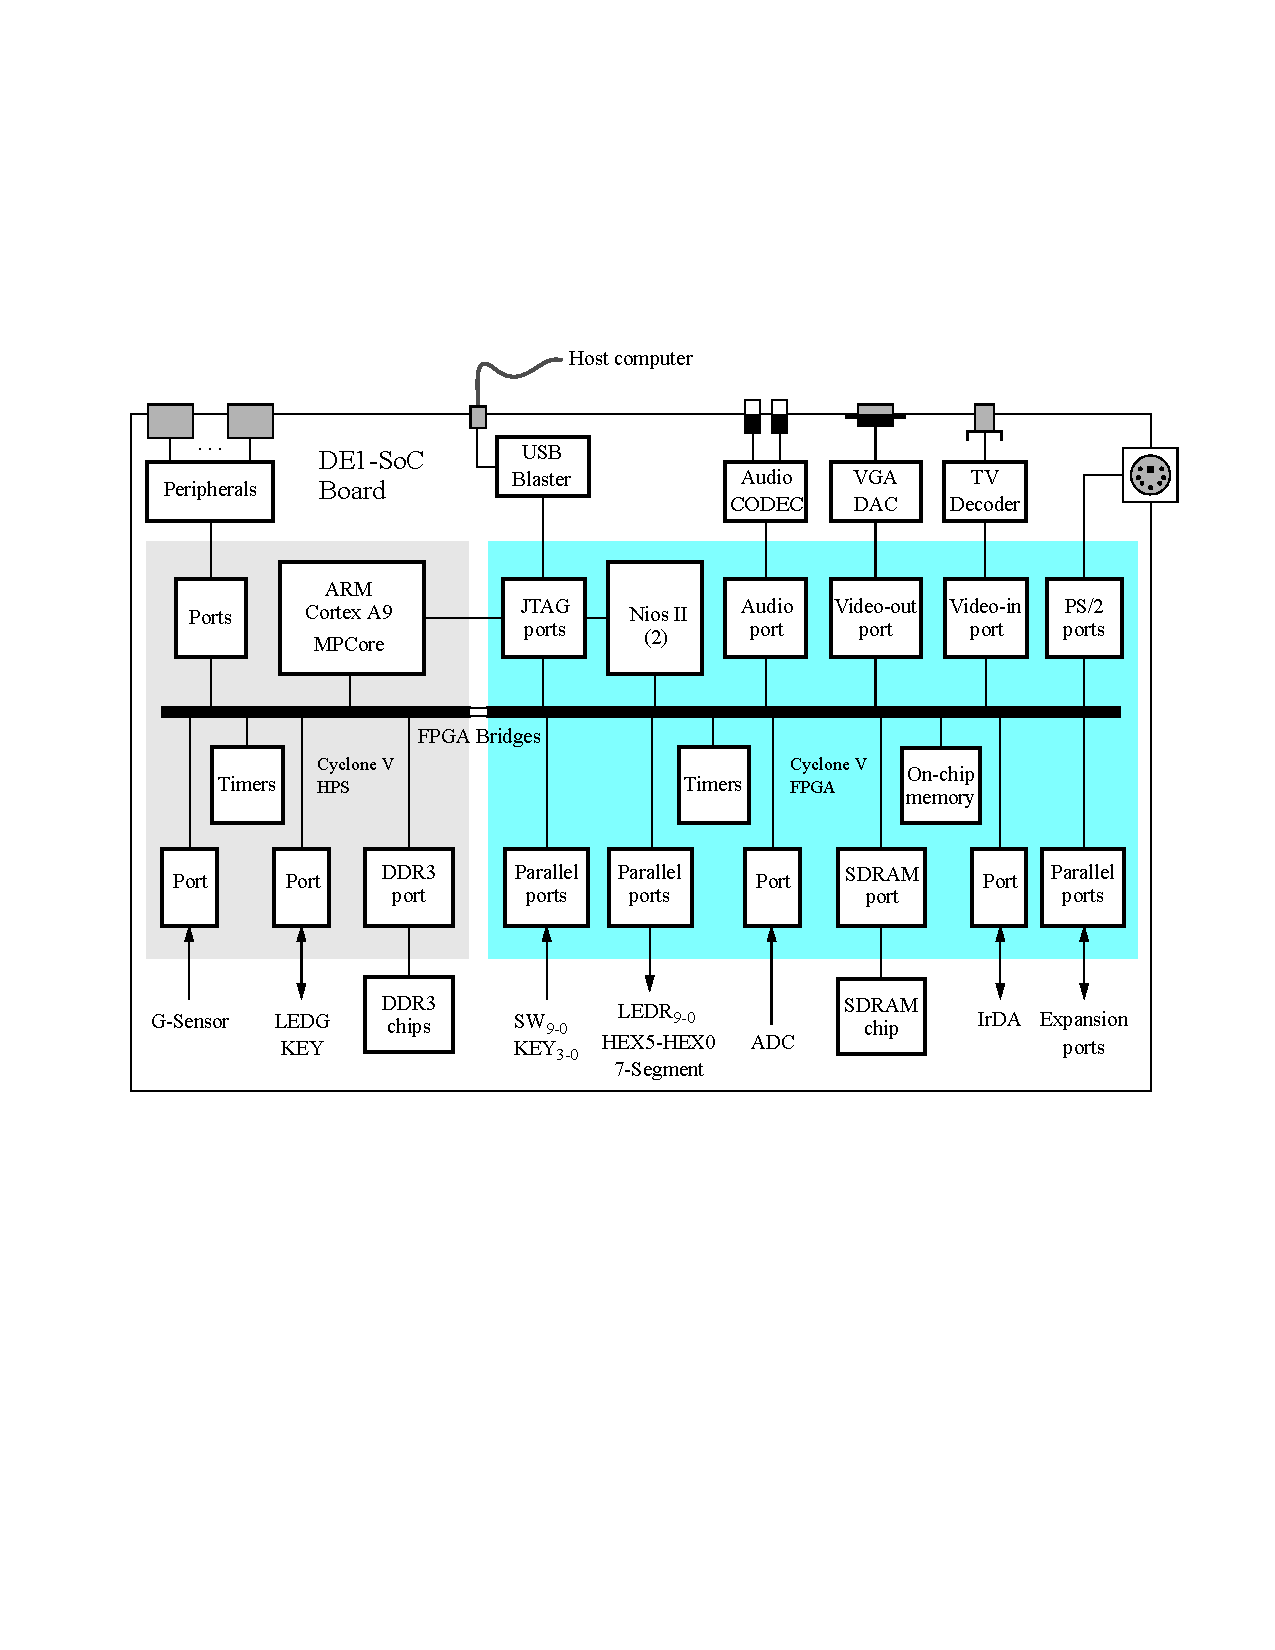
\includegraphics[width=6in]{figures/fig_block_diagram.pdf}
	\caption{System diagram of the DE1-SoC Computer.}
	\label{fig:sys_diagram}
\end{figure}

~\\
\noindent
{\bf Background}

~\\
\noindent
A device driver comprises a set of software subroutines that allow computer programs to access a peripheral device, without the need for the programmer to be familiar with the low-level details of how a peripheral device functions. A simple example of a peripheral device we use in computers is a keyboard, which can be connected to a computer via a PS/2 or a USB interface. Programmers who write a C-language program to read a string of characters from the keyboard on a Personal Computer need not know how keystrokes on the keyboard are received by their program. For example, to read an integer from the keyboard, a C programmer uses the statement:
$$
{\rm scanf("\%d", \&some\_variable);}
$$
\noindent
Providing a high-level of abstraction for peripheral devices is the purpose of device drivers. Implementing device drivers often requires a great deal of knowledge on the part of a programmer, not only with respect to how a peripheral device operates, but also the context in which it is used.

Computer mouse is another example of a simple device that can be connected via a PS/2 or a USB interface. Today, a mouse is likely to be connected using the USB connection. Previously, it was common to use the PS/2 interface. Since the PS/2 interface is much simpler, we will use it in this laboratory exercise.

~\\
\noindent
{\bf Part I}

~\\
\noindent
In this part, you will take the first steps to communicate with the mouse device. To do this, you have to be able to send and receive information from the mouse through the PS/2 port in the DE-series Computer.

The PS/2 port in the Computer is implemented by a PS/2 Port IP core. This core includes a 256-byte First-In First-Out (FIFO) buffer that stores data received from a PS/2 device.

The interface to the PS/2 port in the Computer has two memory-mapped registers, shown in Figure~\ref{fig:ps2_registers}.

\begin{figure}[H]
	\centering
	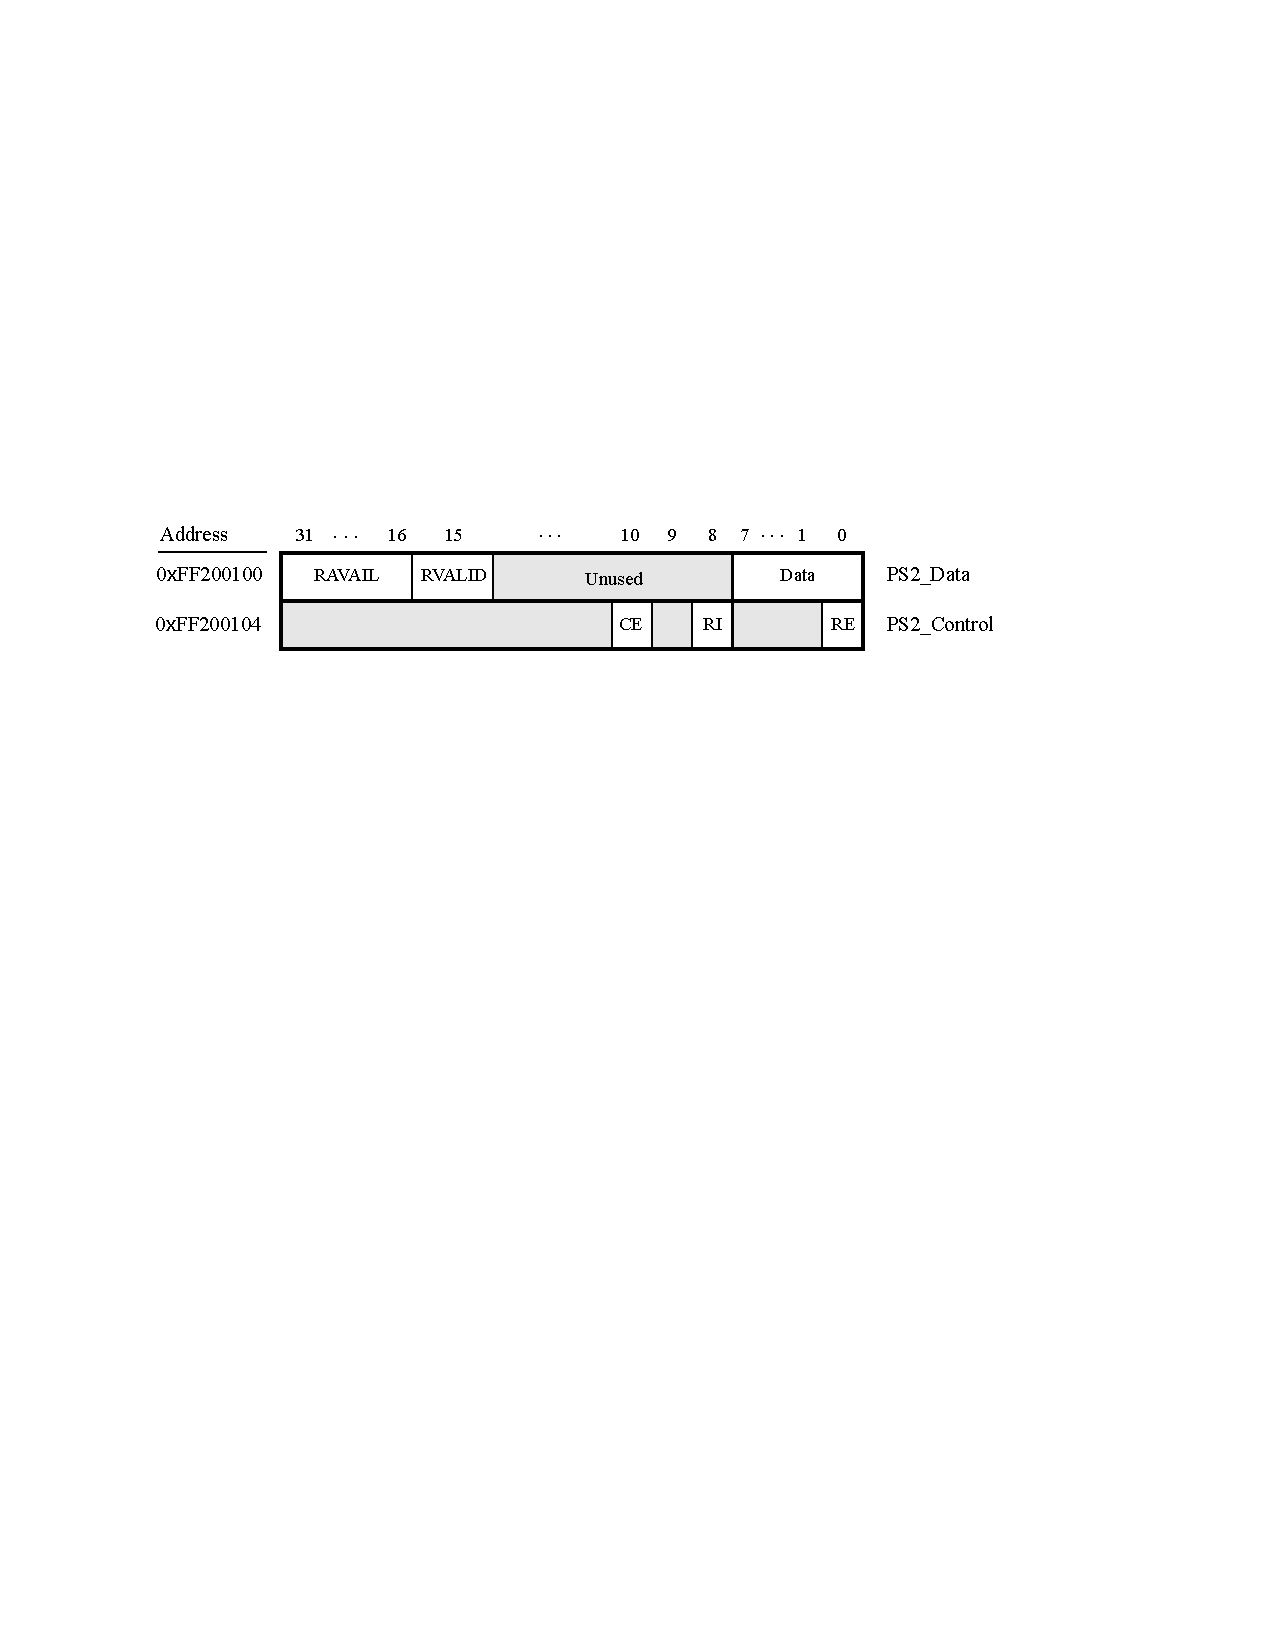
\includegraphics{figures/fig_PS2_port.pdf}
	\caption{PS/2 Port Memory-Mapped Registers.}
	\label{fig:ps2_registers}
\end{figure}

\noindent
The {\sf PS2\_Data} register consists of {\it RAVAIL}, {\it RVALID}, and {\it Data} fields. When {\it RVALID} = 1, the {\it RAVAIL} field indicates the number of
bytes of data received through the PS/2 port that are currently stored in the FIFO buffer. The first byte of the buffer can be read through the {\it Data} field. Note that reading any part of the {\sf PS2\_Data} register causes the FIFO buffer to eject the first byte from the FIFO. The {\sf PS2\_Control} register is used to enable interrupts for the PS/2 port. Interrupts can be enabled by setting the {\it RE} field. When {\it RE = 1}, the PS/2 port generates an interrupt request when {\it RAVAIL} is greater than 0. While the interrupt is pending, the {\it RI} field is set to 1, and can be cleared by emptying the PS/2 FIFO. The {\it CE} field is set by the PS/2 port if an error occurs when a command is sent to a PS/2 device. We will use this register in the later parts of the exercise.

In your first attempt to communicate with the mouse, you will use polling to receive data from the PS/2 port. Do the following:
\begin{enumerate}
	\item Write a C-language program that polls the {\sf PS\_Data} register and displays the last three bytes received on the 7-segment displays. Your program should first enable communication with the mouse by sending the byte {\sf 0xF4} to the {\sf PS\_Data} register. Your program should then continuously read the contents of the {\sf PS2\_Data} register. Each time, check the {\it RVALID} field to determine if the byte in {\it Data} field is valid data. Only when the {\it RVALID} field is 1, should you save the data and display it on the 7-segment displays.
	\item Create a new project in the \productNameMedTM{} for the Intel DE-series Computer and include your source code.
	\item Compile and load your program onto the DE-series board.
	\item Connect a PS/2 Mouse to the PS/2 port on the board.
	\item Run the program and observe the messages received from the mouse device as you move the mouse around and press the mouse buttons.
\end{enumerate}

~\\
\noindent
{\bf Part II}

~\\
\noindent
In this part, you will enhance your program to properly initialize the mouse device. To do this, you will need to understand
some of the commands that can be sent to the mouse (such as the {\sf 0xF4} command we used in Part I), as well as the messages that the mouse can send in response to these commands. The necessary commands and mouse responses to the commands are shown in Table~\ref{tab:mouse_commands}.

\begin{table}[h]
	\caption{Some of the mouse commands along with the expected responses.}
	\begin{center}
	\begin{tabular}{|p{5.5 cm}|p{2 cm}|p{7 cm}|}
	\hline
	\textbf{Command Description} &
	\textbf{Command Byte} &
	\textbf{Response}
	\\\hline
	Reset the mouse to default mode &
	0xFF &
	Responds with a {\bf 0xFA} message, followed by a 2-byte message {\bf 0xAA00} if successful. A byte {\bf 0xFC} will be sent otherwise to indicate an error.
	\\\hline
	Enable Mouse to send position and button status messages &
	0xF4 &
	Responds with a single {\bf 0xFA} byte if successful.
	\\\hline
	Disable Mouse &
	0xF5 &
	Responds with a single {\bf 0xFA} byte if successful. Send the Enable mouse command to resume
	receiving messages about the user's interactions with the mouse.
	\\\hline
	\end{tabular}
	\end{center}
	\label{tab:mouse_commands}
\end{table}

To ensure the proper operation of the mouse device, it is important to reset the mouse and enable it before attempting to process any messages. Thus, your program should first send the reset command to the mouse and await a response. If the reset is successful, the mouse will send a 3-byte sequence equal to {\bf 0xFAAA00}. Upon receiving this response from the mouse, send the {\bf Enable Mouse} command and wait for the acknowledgement {\bf 0xFA}.

Resetting the mouse can fail because of a malfunction, a communication error or because the mouse is not connected to the system. If a mouse malfunctions and does not respond to commands, then it can be treated as not connected. If it responds with the {\bf 0xFC} byte, then resend the reset command to ensure that the mouse is reset correctly before proceeding further.

A disconnected mouse may be reconnected at any time and should be initialized properly. Fortunately, when a mouse is plugged into a PS/2 port it will reset itself and send a 2-byte message {\bf 0xAA00} as though a reset command was sent to it. Your program should watch for the {\bf 0xAA00} message from the mouse. If this sequence is detected, your program should send the reset command to the mouse followed by the mouse enable command.

Write a C-language program that communicates with a mouse through the PS/2 port on the DE-series Computer. Your program should correctly reset and enable the mouse device, as well as handle the case of the mouse being reconnected to the system while the program is running.

~\\
\noindent
{\bf Part III}

~\\
\noindent
In this part, you will learn how to process messages that the mouse device sends to specify the change in its position and the state of its buttons. The change in position is indicated by two 9-bit signed numbers, one for the change in the horizontal position, and one for the change in the vertical position. Moving the mouse to the right causes the horizontal change in mouse's position to be positive, and moving the mouse to the left is indicated by a negative value. Similarly, when you move
the mouse forward, the change in vertical position is positive, and when you pull it towards you it is negative. The state of
mouse buttons is specified using three bits, one per button in a basic 3-button mouse. When a button is pressed the corresponding bit is set to 1, otherwise the bit is set to 0.

By default, a mouse that is enabled will send 3-byte packets through the PS/2 port to communicate its state. The format of the
packet is shown in Table~\ref{tab:mouse_three_byte_packet}.

\begin{table}[h]
	\caption{Three-byte mouse data packet.}
	\begin{center}
		\begin{tabular}{|c|c|c|c|c|c|c|c|c|}
			\hline
			~&
			\textbf{bit 7} &
			\textbf{bit 6} &
			\textbf{bit 5} &
			\textbf{bit 4} &
			\textbf{bit 3} &
			\textbf{bit 2} &
			\textbf{bit 1} &
			\textbf{bit 0}
			\\\hline
			byte 1&
			$y$ overflow &
			$x$ overflow &
			$y$ sign &
			$x$ sign &
			1 &
			Middle btn &
			Right btn &
			Left btn
			\\\hline
			byte 2&
			\multicolumn{8}{|c|}{Mouse $x$ movement}
			\\\hline
			byte 3&
			\multicolumn{8}{|c|}{Mouse $y$ movement}
			\\\hline
		\end{tabular}
	\end{center}
	\label{tab:mouse_three_byte_packet}
\end{table}

\noindent
The first byte has bit 3 set to 1 to indicate that the two bytes to follow are part of a 3-byte data packet. In addition, it contains the state of three buttons in bits 2 through 0, as well as the sign and overflow bits for the movement along the $x$ and $y$ axes. The remaining two bytes contain 8-bit parts of $x$ and $y$ movement of the mouse.

Write a C-language program that initializes the mouse and processes the 3-byte movement packets received from the mouse. Your program should decode the packets and display the state of the buttons on {\bf LEDR[2..0]}, the change in $x$ position on {\bf HEX[5..3]} and the change in $y$ position on {\bf HEX[2..0]}.

~\\
\noindent
{\bf Part IV}

~\\
\noindent
In this part, you will handle the mouse messages using an Interrupt Service Routine. The interrupt service routine (ISR) is a function that is executed when an interrupt occurs. An interrupt will occur when the {\it RE} bit in the PS/2 control register is set to 1 and the PS/2 port has a message ready to be read.

Modify your C-language program from Part III to do this by implementing four functions:
\begin{enumerate}
	\item initialize\_driver - enable the driver to process messages from the mouse. This function should reset the mouse and enable interrupts for the PS/2 port in the DE-series Computer.
	\item disable\_driver - disable the processing of messages from the mouse. Also, disable interrupts for the PS/2 port.
	\item get\_mouse\_change - get the most recent change in position and mouse buttons as reported by the mouse.
	\item PS2\_ISR - the interrupt service routine that handles the mouse events.
\end{enumerate}

Note that the procedure for dealing with interrupts in a DE-series Computer is the subject of Laboratory Exercise 7.

~\\
\noindent
{\bf Part V}

~\\
\noindent
In this part, you will enhance your device driver to keep track of the location of the mouse and limit its movements to specified boundaries. To do this, you will define five variables: two to keep track of the current horizontal and vertical position of the mouse, one to keep the state of mouse buttons, and two to specify the maximum horizontal and vertical coordinates at which the mouse can be located. 

You are to create a mouse device driver comprising the following functions:
\begin{enumerate}
	\item initialize\_driver - as in Part IV.
	\item disable\_driver - as in Part IV.
	\item set\_mouse\_bounds($max_x$, $max_y$) - set the maximum $x$ and $y$ coordinates a mouse can have.
	\item get\_mouse\_state - read the current position of the mouse on the screen and the state of its three buttons.
	\item get\_mouse\_change - as in Part IV.
	\item PS2\_ISR - as in Part IV.
\end{enumerate}

Write a program that shows the position of the mouse using {\bf HEX[5..3]} to display the $x$ position, and {\bf HEX[2..0]} to display the $y$ position. Set the maximum $x$ and $y$ coordinates of the mouse to be 319 and 239, respectively.
 
~\\
\noindent
{\bf Part VI}

~\\
\noindent
In this part, you are to implement routines to draw the mouse pointer on the screen. You will use the VGA cores in the DE-series Computer to draw the mouse pointer on the screen. These cores implement the VGA interface that is able to produce an image on a computer screen at a resolution of 320 by 240 pixels. The image to be drawn on the screen is stored in memory and can be easily changed. Refer to Laboratory Exercise 7 for details that you need to perform the following parts. 

To draw a mouse pointer on the screen, it is necessary to define the shape of the pointer as well as a secondary buffer that contains the contents of the screen beneath the mouse pointer. The shape of the pointer is drawn on the screen just like any other image. You should use the secondary buffer to store the part of the screen on which the mouse is being drawn. Then, when the mouse is moved in the future, you will be able to restore the contents of the screen easily and move the mouse to a new location.

To define the shape of the mouse pointer use a matrix of 16 rows by 8 columns. Each entry in the matrix should contain one of three values:
\begin{enumerate}
	\item $0$ - to indicate that the correpsonding pixel of the mouse pointer is black.
	\item $1$ - to indicate that the correpsonding pixel of the mouse pointer is white.
	\item $-1$ - to indicate that the correpsonding pixel of the mouse pointer is transparent. Transparent pixels are not drawn when the mouse pointer is being drawn.
\end{enumerate}

\noindent
The matrix and the image of the mouse pointer are given in Figure~~\ref{fig:mouse_pointer}. Note that light blue is used to indicate the transparent pixels.

\begin{figure}[H]
	\centering
	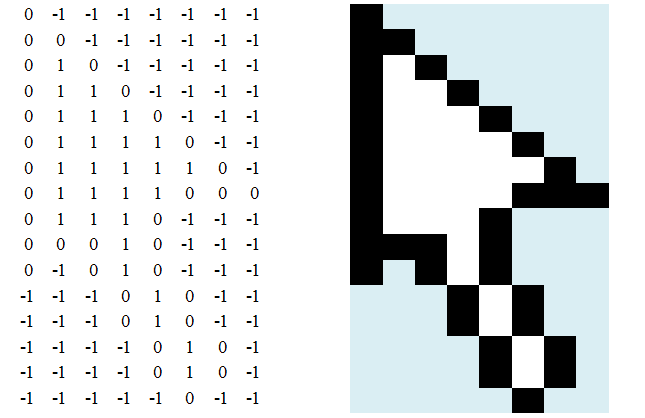
\includegraphics[scale=0.60]{figures/mouse_pointer.png}
	\caption{The matrix and the image of the mouse pointer.}
	\label{fig:mouse_pointer}
\end{figure}

\noindent
The secondary buffer should also consist of 16 rows and 8 columns, where each entry stores the color of the pixel over which the mouse pointer will be drawn.

Adapt your mouse device driver to move the mouse pointer on the screen. Define two new functions for your driver:
\begin{enumerate}
	\item draw\_mouse - store the image underneath the mouse pointer and draw the mouse pointer at the current location. Use the matrix described above to draw the mouse pointer on the screen, assuming that the top-left corner of the mouse pointer image is located at the current location of the mouse. This function should only be visible to the driver.
	\item erase\_mouse - erase the mouse from the screen by redrawing the image beneath the mouse. This function should only be visible to the driver. 
\end{enumerate}

\noindent
Modify your PS/2 Interrupt Service Routine to call the above two functions whenever the mouse position changes.

Run your program from Part V and connect the VGA output of the DE-series board to a computer monitor. You should be able to see
the coordinates of the mouse pointer on the HEX displays and the mouse pointer on the screen, as you move the mouse. 
 
~\\
\noindent
{\bf Part VII}

~\\
\noindent
In this part, you are to combine the mouse pointer with animation on the screen. Write a program to implement a simple game where a filled rectangle moves and bounces off the edges of the screen.  The player moves the mouse to position its pointer on the moving image of the rectangle, at which point clicking the left button on the mouse should change the color of the rectangle and stop its motion. When the button is released, the rectangle should start moving again. The game will be more interesting if you acclerate the speed or shrink the size of the rectangle after each successful catch. 

To perform the animation, every 30th of a second you should hide the mouse pointer, erase the rectangle, draw the rectangle at a new location, and then show the mouse pointer again. You should define two new functions:

\begin{enumerate}
	\item hide\_mouse - causes the driver to erase the mouse from the screen. The driver should still process messages from the mouse, and update its position and the state of the buttons, but the mouse pointer should not be drawn on the screen.
	\item show\_mouse - enables the driver to draw the mouse pointer on the screen. If the pointer was previously hidden, the driver should draw the pointer when this function is called.
\end{enumerate}

To wait a 30th of a second, we can take advantage of the fact the VGA controller continuously redraws the image from the memory
onto the screen and one redraw cycle takes a 60th of a second. We can ask the VGA pixel buffer to let us know when it has finished drawing the most recent image, as explained in Laboratory Exercise 7. Waiting for two such cycles, gives us the 30th of a second delay we seek.

When you run your program you may notice that as you move the mouse pointer, parts of it are left on the screen, despite the fact that you were careful to erase and redraw it in both your ISR and in your main program. The reason is that an interrupt can occur while your main program is hiding/redrawing the mouse. You will need to adjust your driver to prevent this.

~\\
\noindent
{\bf Preparation}

~\\
\noindent
The recommended preparation for this laboratory exercise includes C code for Parts I through VII.


%%%%%%%%%%%%%%%%%%%%%%%%%%%%%%%%%%%%%%%%
%%% FPGAcademy Copyright Information %%%
%%%%%%%%%%%%%%%%%%%%%%%%%%%%%%%%%%%%%%%%

%Always put the copyright on a new page (clear page), with some vertical space from top
\clearpage
\vspace{1in}

\noindent

Copyright {\copyright} FPGAcademy.org. All rights reserved. FPGAcademy and the 
FPGAcademy logo are trademarks of FPGAcademy.org.  This document is provided 
"as is", without warranty of any kind, express or implied, including but not 
limited to the warranties of merchantability, fitness for a particular purpose 
and noninfringement. In no event shall the authors or copyright holders be 
liable for any claim, damages or other liability, whether in an action of 
contract, tort or otherwise, arising from, out of or in connection with the 
document or the use or other dealings in the document.
~\\
~\\
**Other names and brands may be claimed as the property of others.


\end{document}
